\section{Kupfer-PVD}
\label{copperpvd}

Mit Kupfer-PVD wurde ein zweiter Metall-PVD-Prozess auf das Parsivald-Modell angepasst und unter der Zielsetzung simuliert, die Anwendbarkeit verschiedener Potentialparametrisierungen zu prüfen.
Der Prozess ähnelt dem Gold-Prozess in seinen Parametern, jedoch konnten viele verschiedene Parametersätze für Kupferoberflächen, -schmelzen und -legierungen gefunden werden, von denen einige Hinweise auf die Nicht-Darstellbarkeit der reinen Metallsysteme enthalten\cite{mendelev_development_2009}\cite{mendelev_using_2007}.

Aus diesem Grund ist eine einfache Voruntersuchung der verfügbaren Parametersätze notwendig, anhand derer Kandidaten für Parsivald für vollständige Abscheidungssimulationen gesucht werden.

\begin{table}
  \oddrowcolors
  \caption{Untersuchte EAM-Parametrisierungen für Kupfersysteme}
  \label{tab:copperpots}
  \begin{tabularx}{\textwidth}{|lXc|}
    \hline
    \textbf{Bezeichnung}        & \textbf{Anwendung \& Kommentare}                                             & \textbf{Ref.}                            \\
    \hline
    CuAg.eam.alloy              & struktur. und thermodyn. Eigenschaften von \ce{Cu-Ag}                        & \cite{williams_embedded-atom_2006}       \\
    cu\_ag\_ymwu.eam.alloy      & Mono-, Di-, Trimere und Inseln von \ce{Cu} auf \ce{Ag}                       & \cite{wu_cu/ag_2009}                     \\
    Cu\_smf7.eam                & Oberflächen von \ce{Ni-Cu}-Legierungen bei \SI{800}{\kelvin}                 & \cite{foiles_calculation_1985}           \\
    Cu\_u3.eam                  & Oberflächen und Bulks verschiedener Legierungen                              & \cite{foiles_embedded-atom-method_1986}  \\
    Cu\_u6.eam                  & Aktivierungsenergie für Eigendiffusionen                                     & \cite{adams_self-diffusion_1989}         \\
    Cu-Zr\_2.eam.fs             & Flüssige und amorphe \ce{Cu-Zr}-Legierungen                                  & \cite{mendelev_development_2009}         \\
    Cu-Zr.eam.fs                & Flüssige und amorphe \ce{Cu-Zr}-Legierungen                                  & \cite{mendelev_using_2007}               \\
    Mendelev\_Cu2\_2012.eam.fs  & Unterkühlte \ce{Al-Cu}-Schmelzen. Basiert auf \cite{mendelev_analysis_2008}  & \cite{becker_interatomic_2014}                 \\
    \hline
  \end{tabularx}

\end{table}

\subsection{Voruntersuchungen}

Als Vorbetrachtung für die Anwendbarkeit in Abscheidungssimulationen wurden Koordinationszahlen, Bindungslängen und Dichten mit allen Parametersätzen ermittelt und mit experimentellen Daten verglichen.
Die Ergebnisse stimmen im Allgemeinen gut mit experimentellen Werten überein (Tabelle~\ref{tab:copperpreresults}), zeigt aber für cu\_ag\_ymwu.eam.alloy eine Abweichung in der Bindungslänge von \SI{3.25}{\percent}, die zu einer Dichteabweichung von \SI{10.4}{\percent} führt.
Die meisten anderen Parametersätze unterschätzen die Bindungslänge nur leicht, mit Ausnahme der mit LAMMPS vertriebenen Dateien, welche ideale strukturelle Eigenschaften produzieren.
Diese wurden in den weiteren Simulationen aufgrund der guten strukturellen Übereinstimmung sowie ihrer Bewährtheit in Kombination mit LAMMPS zu Rate gezogen.

Mit den Parameterdateien wird der Schmelzpunkt stark überschätzt, mit Ausnahme von cu\_ag\_ymwu.eam.alloy, die den Schmelzpunkt um 300K unterschätzt (Abbildung~\ref{fig:copperthermo}).
Hier zeigt sich die Eigenschaft der Molekulardynamik, jeweils nur für ein enges Anwendungsgebiet passende Ergebnisse zu liefern.
Wie Tabelle~\ref{tab:copperpots} zu entnehmen ist, wurden die verfügbaren Parametersätze nicht für thermodynamische Untersuchungen angepasst und unterstützen diese somit nicht offiziell, doch werden solche extremen Temperaturen in den durchgeführten Simulationen ohnehin nicht erreicht.

\begin{table}
  \begin{threeparttable}
    \oddrowcolors
    \caption{Vergleich struktureller Eigenschaften von Kupfer mit Literaturdaten}
    \label{tab:copperpreresults}
    \begin{tabularx}{\textwidth}{|Xrrrrr|}
      \hline
      \textbf{Parametersatz}      &  \textbf{Koord.}  &  \multicolumn{2}{c}{\textbf{Bindungslänge}}  ~  ~                       &  \textbf{Dichte}    &  ~                       \\
      \hline
      Referenz                    &  \num{12.00}      &  \SI{2.556}{\angstrom}                       &  ~                       &  \SI{8.92}{\gpcc}   &  ~                       \\
      CuAg.eam.alloy              &  \num{12.09}      &  \SI{2.559}{\angstrom}                       &  (\SI{-0.12}{\percent})  &  \SI{8.893}{\gpcc}  &  (\SI{-0.30}{\percent})  \\
      cu\_ag\_ymwu.eam.alloy      &  \num{12.03}      &  \SI{2.473}{\angstrom}                       &  (\SI{-3.25}{\percent})  &  \SI{9.846}{\gpcc}  &  (+\SI{10.4}{\percent})  \\
      Cu\_smf7.eam                &  \num{12.03}      &  \SI{2.558}{\angstrom}                       &  (\SI{+0.08}{\percent})  &  \SI{8.908}{\gpcc}  &  (\SI{-0.13}{\percent})  \\
      Cu\_u3.eam                  &  \num{12.00}      &  \SI{2.558}{\angstrom}                       &  (\SI{+0.08}{\percent})  &  \SI{8.915}{\gpcc}  &  (\SI{-0.06}{\percent})  \\
      Cu\_u6.eam                  &  \num{12.00}      &  \SI{2.558}{\angstrom}                       &  (\SI{+0.08}{\percent})  &  \SI{8.910}{\gpcc}  &  (\SI{-0.11}{\percent})  \\
      CuNi.eam.alloy              &  \num{12.10}      &  \SI{2.559}{\angstrom}                       &  (\SI{-0.12}{\percent})  &  \SI{8.895}{\gpcc}  &  (\SI{-0.28}{\percent})  \\
      Cu-Zr\_2.eam.fs             &  \num{12.05}      &  \SI{2.575}{\angstrom}                       &  (\SI{-0.74}{\percent})  &  \SI{8.738}{\gpcc}  &  (\SI{-2.04}{\percent})  \\
      Cu-Zr.eam.fs                &  \num{12.09}      &  \SI{2.575}{\angstrom}                       &  (\SI{-0.74}{\percent})  &  \SI{8.738}{\gpcc}  &  (\SI{-2.04}{\percent})  \\
      Mendelev\_Cu2\_2012.eam.fs  &  \num{12.07}      &  \SI{2.575}{\angstrom}                       &  (\SI{-0.74}{\percent})  &  \SI{8.747}{\gpcc}  &  (\SI{-1.94}{\percent})  \\
      \hline
    \end{tabularx}

    %% \tnote{a}
    %% \begin{tablenotes}
    %%   \item[a] Der Wert in Klammern ist die Abweichung vom experimentellen Wert
    %% \end{tablenotes}
  \end{threeparttable}
\end{table}

\begin{figure}
  \captionsetup[subfigure]{singlelinecheck=false}
  \def\subfigwidth{7cm}
  \begin{subfigure}[t]{\subfigwidth}
    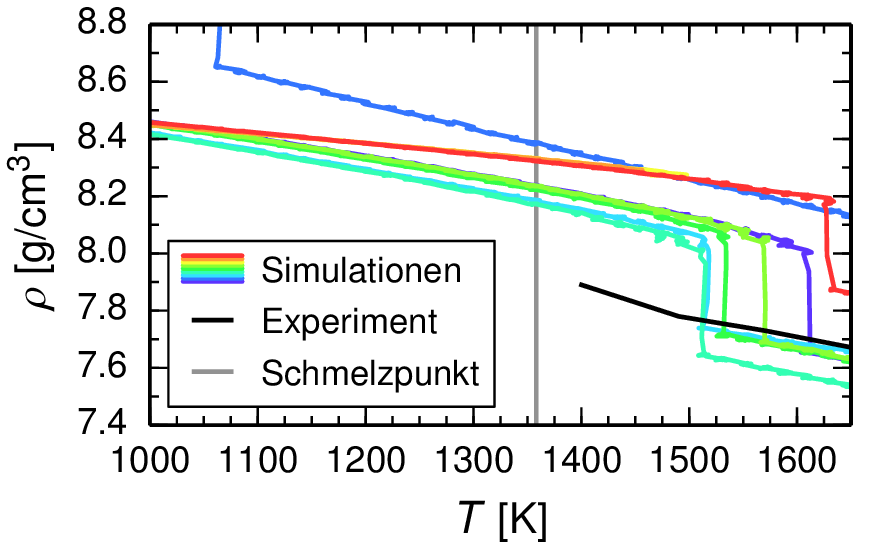
\includegraphics[width=\textwidth]{Cu_trelax_all}
    \subcaption{Schmelzpunkte aller Parametrisierungen}
  \end{subfigure}
  \hfill
  \begin{subfigure}[t]{\subfigwidth}
    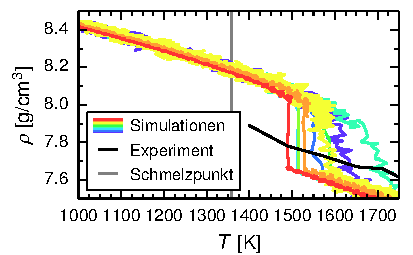
\includegraphics[width=\textwidth]{Cu_smf7_meltingpoint}
    \subcaption{Schmelzpunkte mit smf7 in Abh. von $t_\text{relax}$}
  \end{subfigure}
  \caption[Vergleich der Schmelztemperatur von Kupfer]{
    Vergleich der Schmelztemperatur von Kupfer.
    Experimentelle Dichte: \cite{brillo_density_2006}
  }
  \label{fig:copperthermo}
\end{figure}

\subsection{Prozess-Simulation}
\label{coppersimulation}

\begin{figure}
  \captionsetup[subfigure]{singlelinecheck=false}
  \def\subfigwidth{0.49\textwidth}
  \begin{subfigure}[t]{\subfigwidth}
    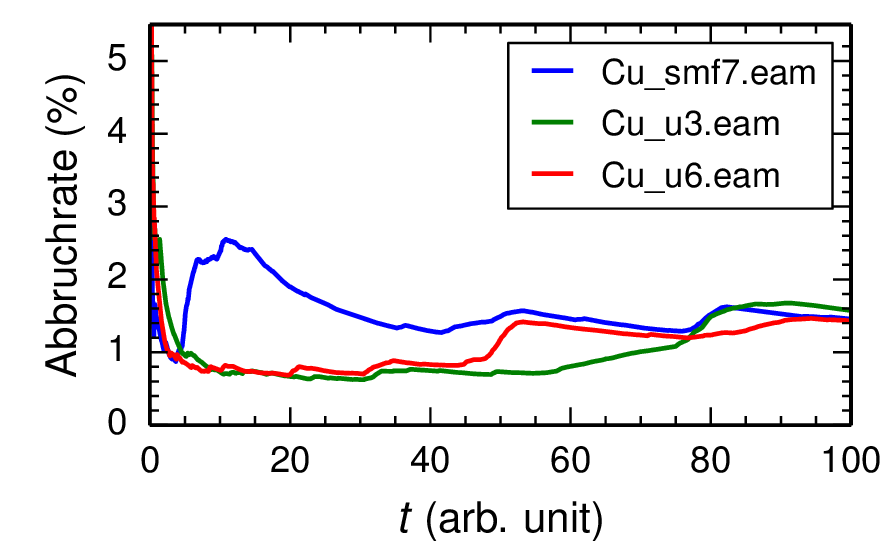
\includegraphics[width=\textwidth]{Cu_abortstatplot}
    \subcaption{Abbruchraten von Kupfer-Simulationen}
    \label{fig:copperparsivald-a}
  \end{subfigure}
  \hfill
  \begin{subfigure}[t]{\subfigwidth}
    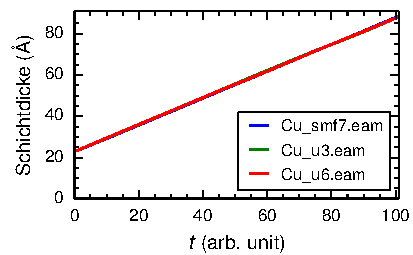
\includegraphics[width=\textwidth]{Cu_thickness}
    \subcaption{Zeitliche Entwicklung der Schichtdicke}
    \label{fig:copperparsivald-b}
  \end{subfigure}
  \begin{subfigure}[t]{\subfigwidth}
    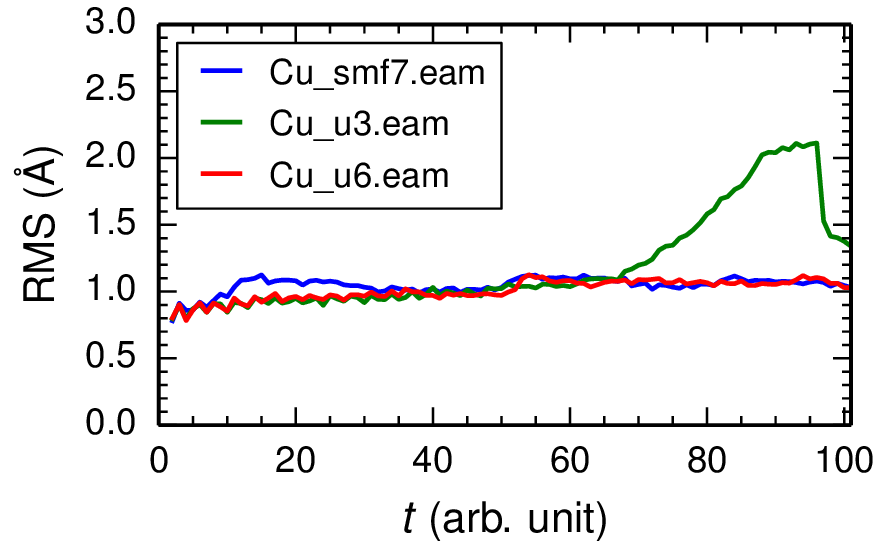
\includegraphics[width=\textwidth]{Cu_roughness}
    \subcaption{Zeitliche Entwicklung der Rauheit}
    \label{fig:copperparsivald-c}
  \end{subfigure}
  \hfill
  \begin{subfigure}[t]{\subfigwidth}
    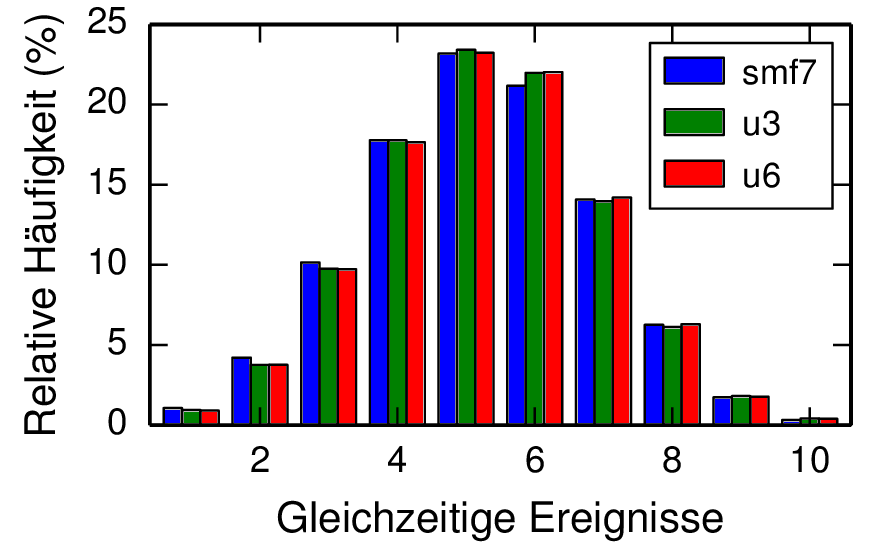
\includegraphics[width=\textwidth]{Cu_eventhistogram}
    \subcaption{Histogramm gleichzeitiger Ereignisse}
    \label{fig:copperparsivald-d}
  \end{subfigure}
  \caption{Simulationen von Kupfer-PVD auf \SI{200x200x24}{\angstrom} großen Substraten}
  \label{fig:copperparsivald}
\end{figure}

In einer PVD-Simulation soll zunächst überprüft werden, ob Kupfer im PVD-Modus von Parsivald fehlerfrei abgeschieden werden kann.
Weiterhin werden die abgeschiedenen Schichten auf Unebenheiten, Fehlstellen und Hohlräume untersucht, um Aussagen über deren Qualität zu gewinnen.
Durch die Ähnlichkeiten zwischen Kupfer und Gold wurden die Prozess-Parameter der Gold-PVD für den Kupfer-Prozess adaptiert.
Unterschiede liegen in den Auftreffenergien von \SI{5.4}{\electronvolt}, die ebenfalls oberhalb experimenteller Werte liegen und vom Thermostat vor dem eigentlichen Auftreffen der Atome auf der Oberfläche noch weiter abgeschwächt werden.

Zu Beginn der einzelnen Simulation ergeben sich extreme Abbruchraten von \SI{25}{\percent}, die durch Herausschlagen einzelner Oberflächenatome bei Ankunft des gesputterten Atomes verursacht werden\todo{Energie trotzdem zu hoch?}.
Bereits nach wenigen Ereignissen sinkt die Abbruchrate auf \SI{3}{\percent}, was auf eine Reduktion des Effektes durch thermische Relaxation und Bedeckung der Oberfläche mit temporären Off-Lattice-Atomen hinweist.
Die kritische Bedeckung dafür liegt zwischen \SI{0.034}{\per\nano\meter\squared} und \SI{0.074}{\per\nano\meter\squared} und deckt sich somit mit der maximalen MD-Ereignisdichte von \SI{0.073}{\per\nano\meter\squared}.
Das deutet darauf hin, dass perfekte Gitterkonfigurationen nicht robust gegenüber gerichteten Energieeinträgen sind, kleine Störungen des Gitters aber zur gleichmäßigeren Verteilung der eingebrachten Energien auf die umliegenden Atome führen.

Im weiteren Verlauf der Simulation liegt die Abbruchrate unterhalb von \SI{2}{\percent} (Abbildung~\ref{fig:copperparsivald-a}), unterliegt aber weiteren Schwankungen, die mit der RMS-Rauheit korrelieren (Abbildung~\ref{fig:copperparsivald-c}), welche durch Unebenheiten der Oberfläche auf der Nanometer-Skala dominiert wird.
Mit einem nahezu konstanten RMS-Wert um \SI{1}{\angstrom} sind die gewachsenen Schichten durchgehend glatt, mit Ausnahme einzelner Simulationen.

Eines der untersuchten Cu\_u3.eam-Systeme bildet ab Schritt 70 einen \SI{2.6}{\nano\meter} breiten und \SI{3.0}{\nano\meter} tiefen Krater aus, der schließlich zu einem \SI{1}{\nano\meter} großen Hohlraum abgeschlossen wird (Abbildung~\ref{fig:coppercrater}).
Die Auswirkungen dieses Kraters auf die Rauheit sind klar in Abbildung~\ref{fig:copperparsivald-c} als stetige Zunahme, gefolgt von einer schlagartigen Abnahme in Schritt 96, und in den Abbruchraten (Abbildung~\ref{fig:copperparsivald-a}) als Anstieg zwischen den Schritten 60 und 90 erkennbar, beeinflussen aber nicht die Wachstumsrate (Abbildung~\ref{fig:copperparsivald-b}).
Das gleiche Verhalten zeigt sich in weiteren Simulationen auch für die anderen Parametersätze und ist nicht auf Cu\_u3.eam begrenzt.

\begin{figure}

  \captionsetup[subfigure]{justification=centering,singlelinecheck=false}
  \def\subfigwidth{0.32\textwidth}

  \begin{subfigure}[t]{\subfigwidth}
    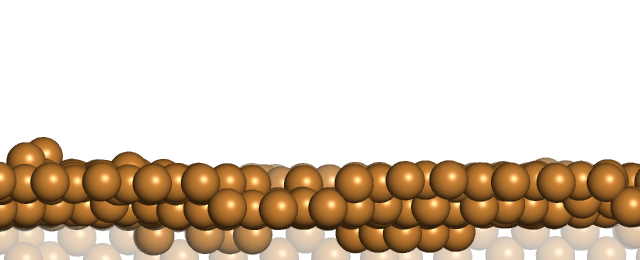
\includegraphics[width=\textwidth]{Cu_crater_01_crop}
    \subcaption{$t=59$}
  \end{subfigure}
  \hfill
  \begin{subfigure}[t]{\subfigwidth}
    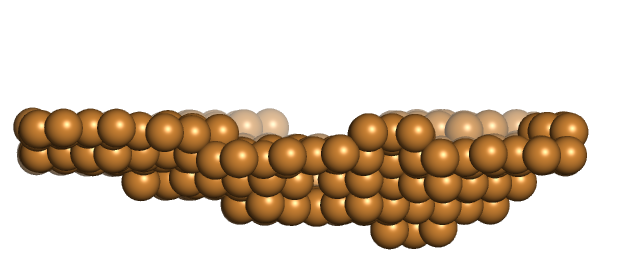
\includegraphics[width=\textwidth]{Cu_crater_07_crop}
    \subcaption{$t=65$}
  \end{subfigure}
  \hfill
  \begin{subfigure}[t]{\subfigwidth}
    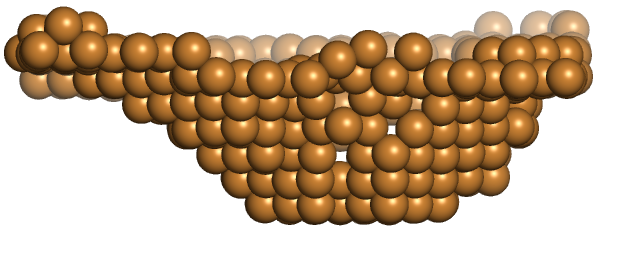
\includegraphics[width=\textwidth]{Cu_crater_17_crop}
    \subcaption{$t=75$}
  \end{subfigure}

  \begin{subfigure}[t]{\subfigwidth}
    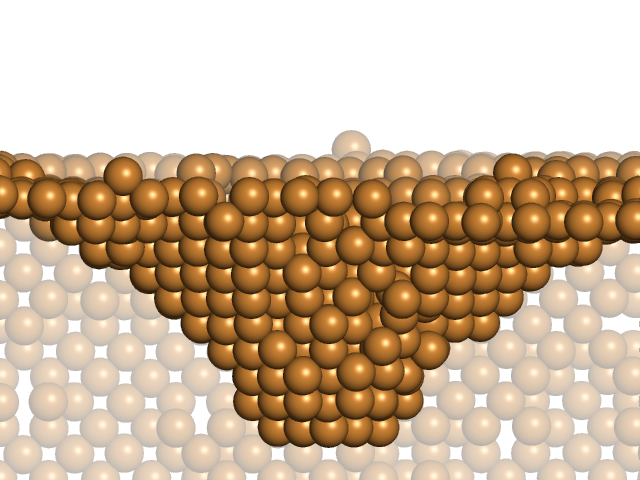
\includegraphics[width=\textwidth]{Cu_crater_27}
    \subcaption{$t=85$}
  \end{subfigure}
  \hfill
  \begin{subfigure}[t]{\subfigwidth}
    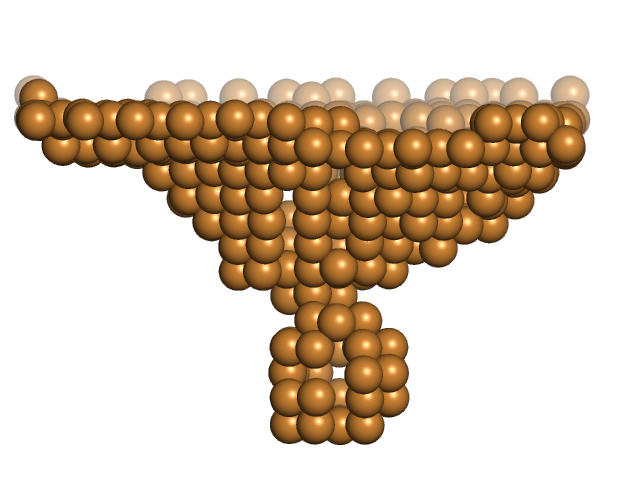
\includegraphics[width=\textwidth]{Cu_crater_37}
    \subcaption{$t=95$}
  \end{subfigure}
  \hfill
  \begin{subfigure}[t]{\subfigwidth}
    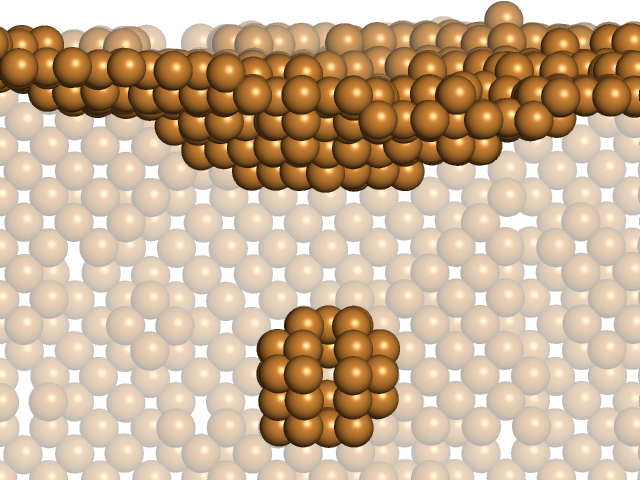
\includegraphics[width=\textwidth]{Cu_crater_42}
    \subcaption{$t=100$}
  \end{subfigure}

  \caption[Bildung und Abschluss eines Kupfer-Kraters]{
    Bildung und Abschluss eines Kupfer-Kraters mit Cu\_u3.eam.\\
    Seitenansicht der extrahierten Oberflächenatome (\SI{30x03}{\angstrom})
  }
  \label{fig:coppercrater}
\end{figure}

\subsubsection{Maximale Ereignisdichte}
Ergänzend ist in Abbildung~\ref{fig:copperparsivald-d} ein Histogramm der Zahl paralleler Ereignisse dargestellt.
Die maximale Oberflächendichte der Ereignisse liegt bei der gewählten MD-Box-Größe von \SI{37x37}{\angstrom} bei \SI{0.073}{\per\nano\meter\squared}.
Dem stehen beobachtete Maxima von \num{12} aktiven Ereignissen gegenüber, die einer Dichte von \SI{0.03}{\per\nano\meter\squared} und somit \SI{40}{\percent} maximaler Bedeckung entsprechen, wobei im Schnitt nur \num{5.3} Worker aktiv sind, was einer mittleren Bedeckung von \SI{18.5}{\percent} entspricht.
Die Bedeckungsdichten für Systeme unterschiedlicher Größe wurden bereits in Tabelle~\ref{tab:goldscalability} für Gold-Abscheidungen aufgelistet und zeigen ähnliche Werte für kleine Systeme, können für Substrate auf der Mikrometer-Skala mangels verfügbarer Rechenleistung jedoch nicht aufrecht erhalten werden.
